\section{Mô phỏng giao diện kiểm tra khuyết tật màn hình thời gian thực}
Giao diện ứng dụng mô phỏng kiểm tra khuyết tật màn hình thời gian thực được phát triển nhằm trực quan hóa các chỉ số vận hành và cấu trúc mạng tự điều chỉnh của mô hình EAGNG trong quá trình xử lý dòng dữ liệu. Hệ thống giao diện tích hợp trực tiếp luồng xử lý ảnh với mạng nơ-ron học trực tuyến, giúp giám sát các tham số phân cụm và thời gian đáp ứng của mô hình ở từng bước thời gian. Cấu trúc giao diện được chia thành các khu vực chức năng chính bao gồm (i) khung hiển thị ảnh kiểm tra và kết quả nhận dạng, (ii) khung biểu diễn đồ thị cấu trúc topology của mạng EAGNG, (iii) khung đo lường các chỉ số hiệu năng phân cụm thời gian thực, và (iv) khung quản lý tiến trình thực nghiệm đối sánh. Việc phân chia cấu trúc này bảo đảm tính minh bạch trong quá trình theo dõi sự biến đổi cấu trúc mạng khi xuất hiện hiện tượng trôi dạt khái niệm trên dòng dữ liệu.

Khung hiển thị hình ảnh kiểm tra nằm ở góc trên bên trái thể hiện trực tiếp mẫu ảnh đang được nạp vào hệ thống cùng thông tin phân loại chi tiết. Trong Hình \ref{fig:c4_app_demo}, mẫu ảnh thứ 1246 trên tổng số 3000 mẫu đại diện cho khuyết tật dạng hình tam giác được đưa vào xử lý và thu được kết quả nhận dạng chính xác. Ngay bên cạnh, khung biểu diễn đồ thị mạng EAGNG trực quan hóa sự phân bố không gian của 268 nút mạng cùng 51 liên kết cạnh giữa các nút. Đồ thị cấu trúc phản ánh sự hình thành của các cụm dữ liệu phân biệt từ C0 đến C7, trong đó số lượng cụm hoạt động duy trì ở mức bốn cụm chính tương ứng với các phân bố đặc trưng đã tích lũy. Việc hiển thị trực quan đồ thị topology giúp quan sát sự dịch chuyển của các nút mạng và phản ứng thích ứng cấu trúc khi mẫu dữ liệu mới thuộc lớp tam giác xuất hiện.

\begin{figure}[htbp]
\centering
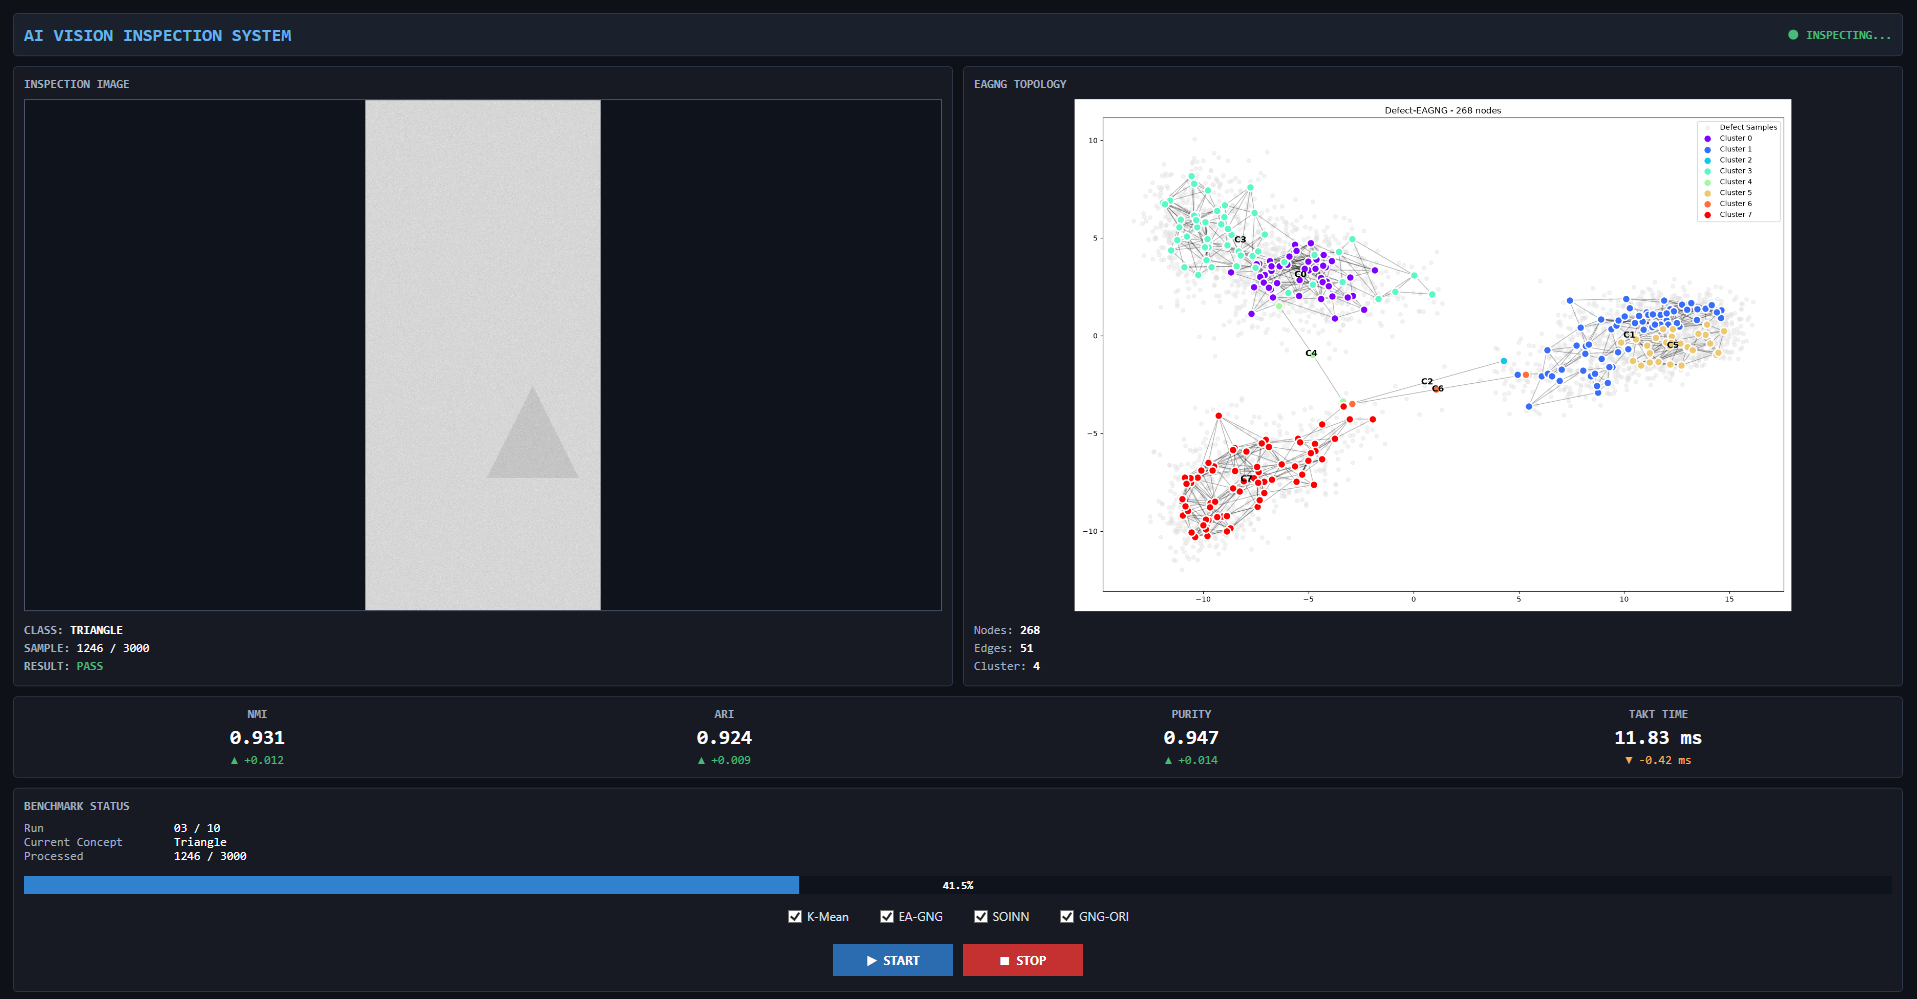
\includegraphics[width=0.98\textwidth]{figures/c4/c4_AppDemo.png}
\caption{Giao diện ứng dụng mô phỏng kiểm tra khuyết tật màn hình thời gian thực trên mạng EAGNG.}
\label{fig:c4_app_demo}
\end{figure}

Khung đo lường chỉ số thời gian thực và quản lý tiến trình thực nghiệm nằm ở phía dưới cung cấp các thông số định lượng cập nhật theo từng mẫu dữ liệu. Kết quả ghi nhận tại thời điểm xử lý mẫu thứ 1246 đạt chỉ số NMI là 0,931, chỉ số ARI đạt 0,924 và độ tinh khiết Purity đạt 0,947. Thời gian nhịp sản xuất Takt Time duy trì ở mức 11,83 millisecond trên một mẫu, khẳng định khả năng đáp ứng yêu cầu vận hành thời gian thực trên dây chuyền công nghiệp. Khung quản lý tiến trình ở đáy giao diện ghi nhận lượt chạy thứ ba trên tổng số mười lượt thực nghiệm với tiến độ hoàn thành đạt 41,5 phần trăm cho kịch bản trôi dạt khái niệm dạng hình tam giác. Hệ thống cho phép kích hoạt đồng thời các thuật toán đối sánh bao gồm K-Means, EAGNG, SOINN và GNG-ORI để so sánh hiệu năng trực tiếp dưới cùng một điều kiện dòng dữ liệu đầu vào \cite{fritzke1995growing, furao2006soinn}.

Mô hình giao diện vận hành ổn định và không xảy ra hiện tượng tắc nghẽn dữ liệu trong suốt chuỗi kiểm thử 3000 mẫu. Tần số cập nhật giao diện được tối ưu hóa thông qua cơ chế bất đồng bộ giữa luồng tính toán mô hình và luồng hiển thị đồ họa. Mức tiêu tốn tài nguyên hệ thống duy trì ở ngưỡng an toàn, đáp ứng tiêu chuẩn triển khai thực tế trên các thiết bị máy tính công nghiệp. Sự suy giảm thời gian nhịp sản xuất xuống mức 11,83 millisecond minh chứng cho hiệu quả của cơ chế hoãn chèn nút và rào chắn mật độ cục bộ trong việc tối ưu hóa chi phí tính toán khoảng cách Euclid.